\documentclass[xcolor=dvipsnames,pdf,10pt]{beamer}
\usetheme{inf-ufrgs}

%%% Encoding and Fonts
\usepackage[utf8]{inputenc}
\usepackage[T1]{fontenc}
\usefonttheme{professionalfonts}
\usepackage{lmodern}
\usepackage[small]{eulervm}


%%% EASY ENUMERATIONS
\newcommand{\bi}{\begin{itemize}}
\newcommand{\ei}{\end{itemize}}
\newcommand{\be}{\begin{enumerate}}
\newcommand{\ee}{\end{enumerate}}
\newcommand{\bd}{\begin{description}}
\newcommand{\ed}{\end{description}}
\newcommand{\tm}{\item}

%%% THEOREMS, DEFINITIONS, ETC... 
\newcommand{\defn}{\textcolor{blue}{\textbf{\textrm{Definition\ }}}}
\newcommand{\thm}{\textcolor{OliveGreen}{\textbf{\textrm{Theorem\ }}}}
\newcommand{\lem}{\textcolor{OliveGreen!50!red}{\textbf{\textrm{Lemma:\ }}}}
\newcommand{\crlr}{\textcolor{green!50!orange!80!black}{\textbf{\textrm{Corolary:\ }}}}
\newcommand{\prf}{\textcolor{Red}{\textbf{\textrm{Proof:\ }}}}
\newcommand{\exmp}{\textcolor{WildStrawberry}{\textbf{\textrm{Example:\ }}}}
\newcommand{\rmk}{\textcolor{Purple}{\textbf{\textrm{Remark:\ }}}}
\newcommand{\excs}{\textcolor{Brown}{\textbf{\textrm{Exercise:\ }}}}
\newcommand{\qstn}{\textcolor{WildStrawberry!90!black}{\textbf{\textrm{Question:\ }}}}
\newcommand{\ansr}{\textcolor{violet}{\textbf{\textrm{Answer:\ }}}}
\newcommand{\grule}{$p = (L \leftarrow K \rightarrow R) $}
\newcommand{\rulesequence}{$p_0,\ldots,p_{n-1},p_n$}
\newcommand{\notn}{\textcolor{gray!50!black}{\textbf{\textrm{Notation:\ }}}}


%%%%%%%%%%%%%%%%%%%%%%%%%%%%%%%%%%%%%%%%%%%%%%%%%%%%%%%%%%%%%%%%%%%%%%%%%%%%%%%%%%%%
\title     [Construction of Concurrent Rules with NACs]      {Construction of Concurrent Rules with NACs}
\author    [Author]                    {Jonas S. Bezerra\\ \texttt{jsbezerra@inf.ufrgs.br}}
\institute                             {\inftitle} 
\date                                  {\today}
%%% O texto entre [ ] vai aparecer na barra inferior...

\renewcommand{\contentstitle}{Outline of this talk}  
%%% Título usado nos slides de seção introduzidos automaticamente
%%%%%%%%%%%%%%%%%%%%%%%%%%%%%%%%%%%%%%%%%%%%%%%%%%%%%%%%%%%%%%%%%%%%%%%%%%%%%%%%%%%%

\usepackage{listings}
\lstset{language=Java,basicstyle=\ttfamily}

\begin{document}

\titlepageINF

\tableofcontentsINF

\section{Negative Application Condition}

\begin{frame}[allowframebreaks]{Negative Application Conditions}
\defn (NAC): A \emph{negative application condition} or $NAC(n)$ on $L$ is an arbitrary graph morphism $n : L \rightarrow N$.\\


\defn (NAC satisfiability): A graph morphism $g: L \rightarrow G$ satisfies $NAC(n)$ on $L$, written $g \models NAC(n)$, iff $\nexists q : N \rightarrow G$ such that $q$ is injective and $q \circ n = g$

\begin{figure}[htbp]
\centering
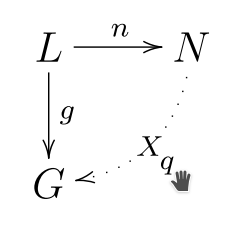
\includegraphics[width=.4\textwidth]{fig/nac-satis.png}
\label{fig:nac-satis}
\end{figure}

\begin{itemize}
\item A set of NACs on $L$ is denoted by $NAC_L = \{NAC(n_i) | i \in I\}$.  A graph morphism $g : L \rightarrow G$ satisfies $NAC_L$ if and only if $g$ satisfies all single NACs on $L$ i.e. $g \models NAC(n_i) \forall i \in I$.
%\item  Se fer tempo colocar a NAC direita e o conujunto de NACs da regra
\end{itemize}

\begin{figure}[htbp]
\centering
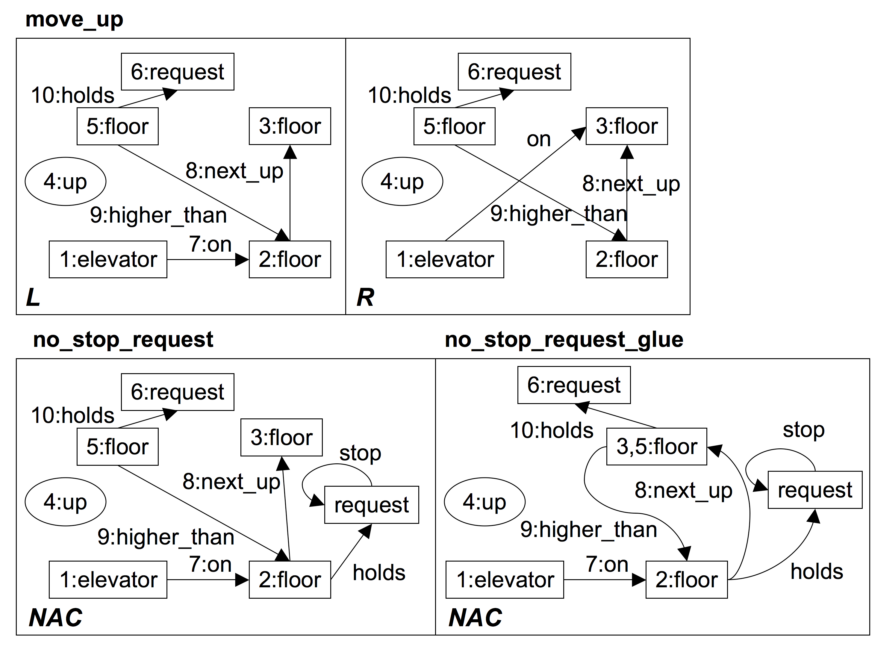
\includegraphics[width=1\textwidth]{fig/injective-nac-example.png}
\caption{\label{fig:shift-right-to-left} Injective NACs example}.
\end{figure}

\end{frame}

\begin{frame}[allowframebreaks]{Different NAC satisfaction and AGG approach}

\begin{itemize}
\item The \emph{definition} demands the non-existing morphism to be injective.
\item Another interpration of NACs the satisfaction of NACs demands the morphism $q: N \rightarrow G$ to be non-injective only on $N \backslash n(L)$. (See Remark 2.3.4)
\item With this interpretation $q$ may glue the same parts as the match is gluing.
\item Without this, for each kind o potential gluing of the LHS, a corresponding NAC needs to be added.

%\item  Se fer tempo colocar a NAC direita e o conujunto de NACs da regra
\end{itemize}

\end{frame}

%%%%%%%%%%%%%%%%%%%%%%%%%%%%%%%%%%%%%%%%%%%%%%%%%%%%%%%%%%

\section{Shifting NACs}

\begin{frame}[allowframebreaks]{Over a Rule}

\defn (construction of Left from right NACs): For each $NAC(n_i)$ on $R$ with $n_i : R \rightarrow N_i$ of a rule $p = (L \leftarrow K \rightarrow R)$, the equivalent left application condition $L_p(NAC(n_i))$ is defined in the following way:

\begin{figure}[htbp]
\centering
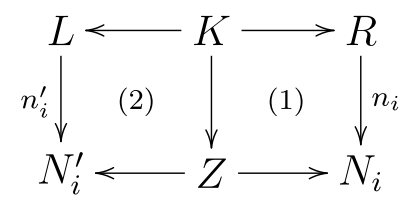
\includegraphics[width=.4\textwidth]{fig/nac-left-from-right.png}
\label{fig:nac-left-from-right}
\end{figure}

\begin{itemize}
\item If the pair $(K \rightarrow R, R \rightarrow N_i)$ has a pushout complement complement, we construct $(K \rightarrow Z, Z \rightarrow N_i)$ as the pushout complement (1). Then we construct pushout (2) with the morphism $n'_i : L \rightarrow N'_i$. Now we define $L_p(NAC(n_i)) = NAC(n'_i)$.
\item If the pair $(K \rightarrow R, R \rightarrow N_i)$ does not have a pushout complement, we define $L_p(NAC(n_i)) = true$
\end{itemize}

\thm (inverse direct transformation with NACs): For each direct transformation with NACs $G \Rightarrow H$ via a rule \grule with $NAC_p$ a set of left NACs on $p$, there exists an inverse direct transformation with NACs $H \Rightarrow G$ via the inverse rule $p^{-1}$ with $NAC_{p^{-1}}$ 

\begin{figure}[htbp]
\centering
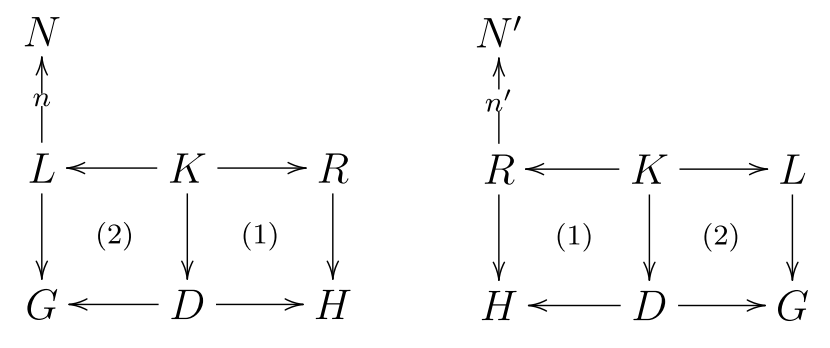
\includegraphics[width=.8\textwidth]{fig/inverse-direct-transformation-with-nacs.png}
\label{fig:inverse-direct-transformation-with-nacs}
\end{figure}

\begin{figure}[htbp]
\centering
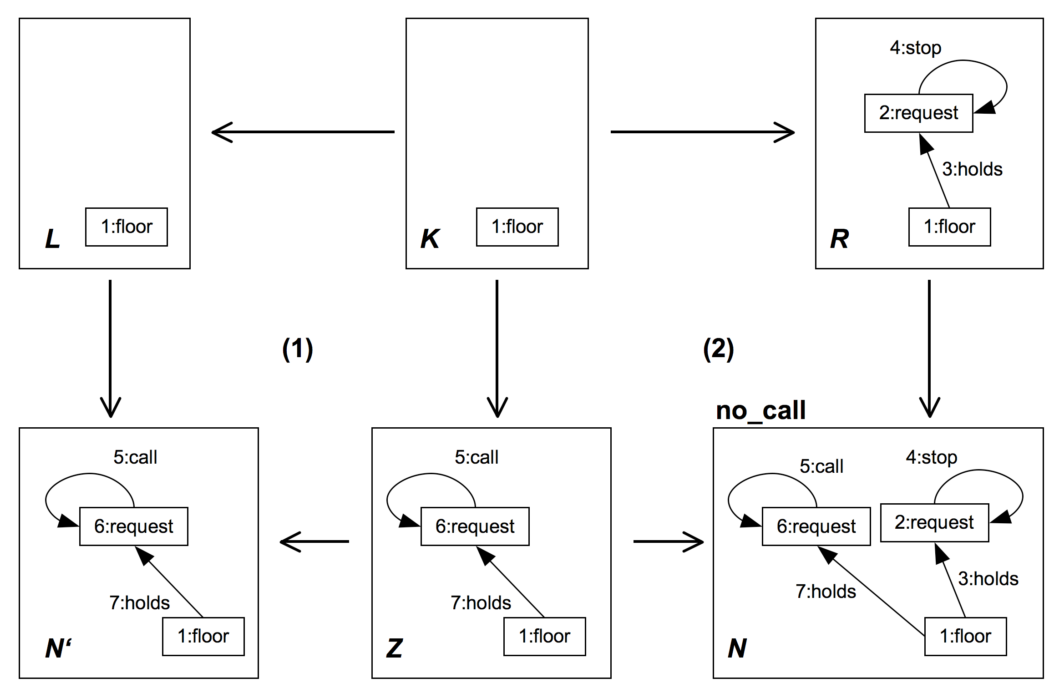
\includegraphics[width=1\textwidth]{fig/shift-right-to-left.png}
\caption{\label{fig:shift-right-to-left} Shifting right NAC into left NAC for Elevator example}.
\end{figure}

\end{frame}

\begin{frame}[allowframebreaks]{Over a Morphism}

\begin{itemize}
\item Consider a graph $A$ with NACs, and some graph morphism $m : A \rightarrow B$.
\item It is not enough to consider the PO of $m$ and the single NACs on A in order to obtain the equivalent NACs on B.
\item All overlaps have to be considered, where in addition graph elements not stemming from $A$ may be glued. 
\end{itemize}

\defn (construction of NACs on $B$ from NACs on $A$ with $m \rightarrow B$). Consider the following diagram: 

\begin{figure}[htbp]
\centering
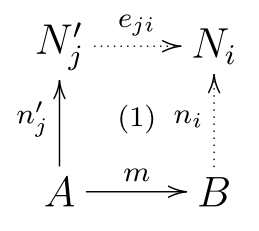
\includegraphics[width=.4\textwidth]{fig/nac-shifted-over-morphism.png}
\label{fig:nac-shifted-over-morphism}
\end{figure}

\begin{figure}[htbp]
\centering
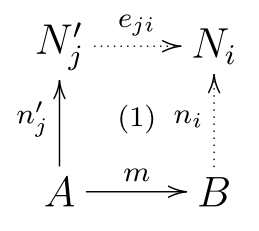
\includegraphics[width=.35\textwidth]{fig/nac-shifted-over-morphism.png}
\label{fig:nac-shifted-over-morphism}
\end{figure}

For each $NAC(n'_j)$ on $A$ with $n'_j : A \rightarrow N'_j$ and $m : A \rightarrow B$, let 

\begin{center}
$D_m(NAC(n'_j)) = \{ NAC(n_i)|i \in I, n_i : B \rightarrow N_i \}$
\end{center}

where $I$ and $n_i$ are constructed as follows:

\begin{itemize}
\item $i \in I$ iff $(e_{ji}, n_i)$ with $e_{ji} : N'_j \rightarrow N_i$ jointly surjective 
\item $e_{ji} \circ n_i = n_i \circ m$
\item $e_ji$ injective
\end{itemize}

For each set of NACs $NAC_A = {NAC(N_j)| j \in J}$ on A the downward shift of $NAC_A$ is then defined as: 

\begin{center}
$D_m(NAC_A) = \cup_{j \in J}D_m(NAC(n'_j))$
\end{center}

$D_m$ is also called the \emph{Downward shift of $NAC_A$}

%% EQUIVALENCE OF SET OF NACS ON A AND B

%% Restriction in the injective case

\begin{figure}[htbp]
\centering
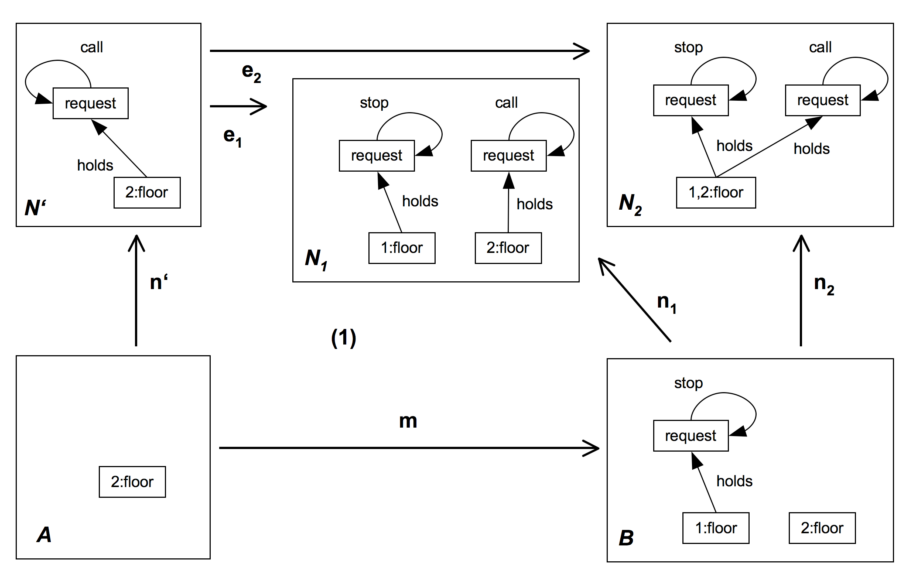
\includegraphics[width=1\textwidth]{fig/nac-shifted-over-morphism-elevator.png}
\caption{\label{fig:nac-shifted-over-morphism-elevator} Example of shifting a NAC over a morphism}.
\end{figure}

\end{frame}

\section{Concurrent rules for a rule sequence}

\begin{frame}[allowframebreaks]{Concurrency}

Let $t$ be a transformation via some rule sequence $p_0,\ldots,p_{n-1}, p_n$ with matches $g_0,\ldots,g_{n-1},g_n$ and sets of NACs $NAC_{p_O},\ldots, NAC_{p_{n-1}}, NAC_{p_n}$:

\begin{itemize}
\item In general there will be casual dependencies, so that is not always possible to summarize the transformation sequence via the \emph{Parallelism Theorem}.
\item It is possible to formulate a \emph{Concurrency Theorem} expressing how to summarize such a sequence into one equivalent transformation step via a concurrent rule.  
\end{itemize}

\end{frame}

\begin{frame}[allowframebreaks]{Without NACs}
\defn (concurrent rule for a rule sequence):

\begin{itemize}
\item $n = 0$ The \emph{concurrent rule} $p_c$ for $p_0$ is $p_0$ itself.
\item $n \geqslant 1$ A concurrent rule $p_c$ for the rule sequence \rulesequence is defined by $p_c = (l \circ k_c : K \rightarrow L, r \circ k_n : K \rightarrow R)$ as show in the following diagram, where 
  \begin{itemize}
  \item $p'_c : L'_c \leftarrow K'_c \rightarrow R'_c$ is a concurrent rule for the sequence $p_0,\ldots,p_{n-1}$
  \item $(e'_c,e_n)$ is jointly surjective
  \item (1), (2), (3) and (4) are pushouts
  \item (5) is a pullback
  \end{itemize}
\end{itemize}

\begin{figure}[htbp]
\centering
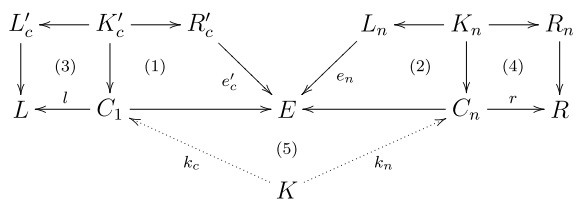
\includegraphics[width=1\textwidth]{fig/concurrent-rule.png}
\caption{\label{fig:concurrent-rule}Construction of a concurrent rule without NACs.}
\end{figure}

\begin{itemize}
\item The concurrent rule $p_c$ may also be denoted as $p'_c \ast_E p_n$.
\end{itemize}

\end{frame}

\begin{frame}[allowframebreaks]{With NACs}

\defn (concurrent rule with NACs for a rule sequence):

\begin{itemize}
\item $n = 0$ The \emph{concurrent rule} $p_c$ with NACs for rule $p_0$ with NACs is $p_0$ with NACs itself.
\item $n \geqslant 1$ A concurrent rule $p_c = p'_c \ast_E p_n $ with NACs for the rule sequence \rulesequence is defined recursively as in the definition without NACs and equals $p_c = (l \circ k_c : K \rightarrow L_c, r \circ k_n : K \rightarrow R)$ 
\end{itemize}

\begin{figure}[htbp]
\centering
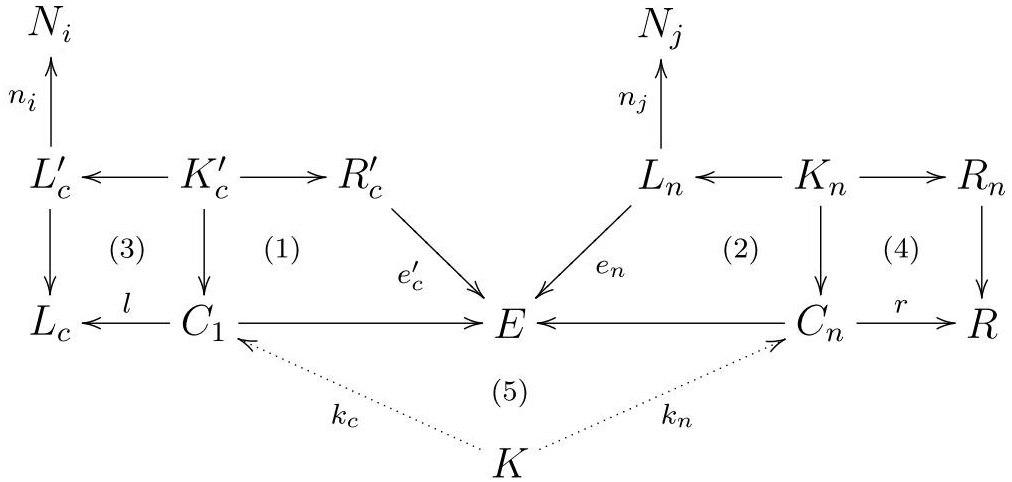
\includegraphics[width=.8\textwidth]{concurrent-rule-with-nac.jpg}
\caption{\label{fig:concurrent-rule-with-nac}Construction of a concurrent rule with NACs.}
\end{figure}

with

\begin{itemize}
\item $NAC_{p_c} = DL_{p_c}(NAC_{L_n}) \cup D_{m_c} (NAC_{L'_c})$ where:
\begin{itemize}
\item $D_{m_c}(NAC_{L'_c})$ is the Downward shift NAC over $m_c : L'_c \rightarrow L_c$
\item $DL_{p_c}(NAC_{L_n})$ with $NAC_{L_n} = \{ NAC(n_j)|j \in J\}$ constructed as follows:
\end{itemize}
\end{itemize}

\begin{center}
$DL_{p_c}(NAC_{L_n}) = \cup_{j \in J}DL_{p_c}(NAC(n_j)) = \cup_{j\in J}L_p(D_{e_n}(NAC(n_j)))$
\end{center}

with 
\begin{itemize}
\item $p = L_c \leftarrow C_1 \rightarrow E$ 
\item $D_{e_n}$ is the Downward shift NAC over $e_n : L_n \rightarrow E$
\item $L_p$ is the left shift NAC over rule $p$
\end{itemize}


\end{frame}

\begin{frame}{References}
\begin{thebibliography}{XX}
\bibitem[Lambers]{1} {\emph{Lambers, Leen. (2010). Certifying Rule-Based Models using Graph Transformation. Elektrotechnik und Informatik der Technischen Universitat Berlin.} \url{https://depositonce.tu-berlin.de/handle/11303/2645}}
\end{thebibliography}
\end{frame}
%----------------------------------------------------------------------------------%



\titlepageINF


\end{document}
